\subsubsection{Stored Files and Source Evidence}
\label{sec:conceptual-files}
StoredFile holds storage metadata shared by document contents, captured signatures
and source evidence. SourceAttachment links one stored file to exactly one ticket,
analysis or valuation; the three target relationships are exclusive alternatives.
This keeps source evidence independent of worker-document version retention.
Figure~\ref{fig:er-source-files} shows the exclusive attachment targets.

File access is authorised through the associated business record, never the storage
key alone. There is no global deduplication or cross-workspace reuse. Remove content
only after releasing retained references. An explicit attachment replacement keeps the old file until the new file is fully stored and validated, then switches the reference and deletes the previous file without history under \decisionref{Q-AT-02}. Failed uploads preserve the old evidence. Prepared-file protection remains under
\decisionref{Q-DOC-07}.

Apply the complete-file consultation and upload grants in
Section~\ref{sec:permission-defaults}. A complete ticket may expose printed monetary
values; consultation grants must therefore be configured consistently. Changing or
removing a link cannot grant another account access to its file. Worker-document
upload remains a separate operation.

\begin{figure}[!htbp]
\centering
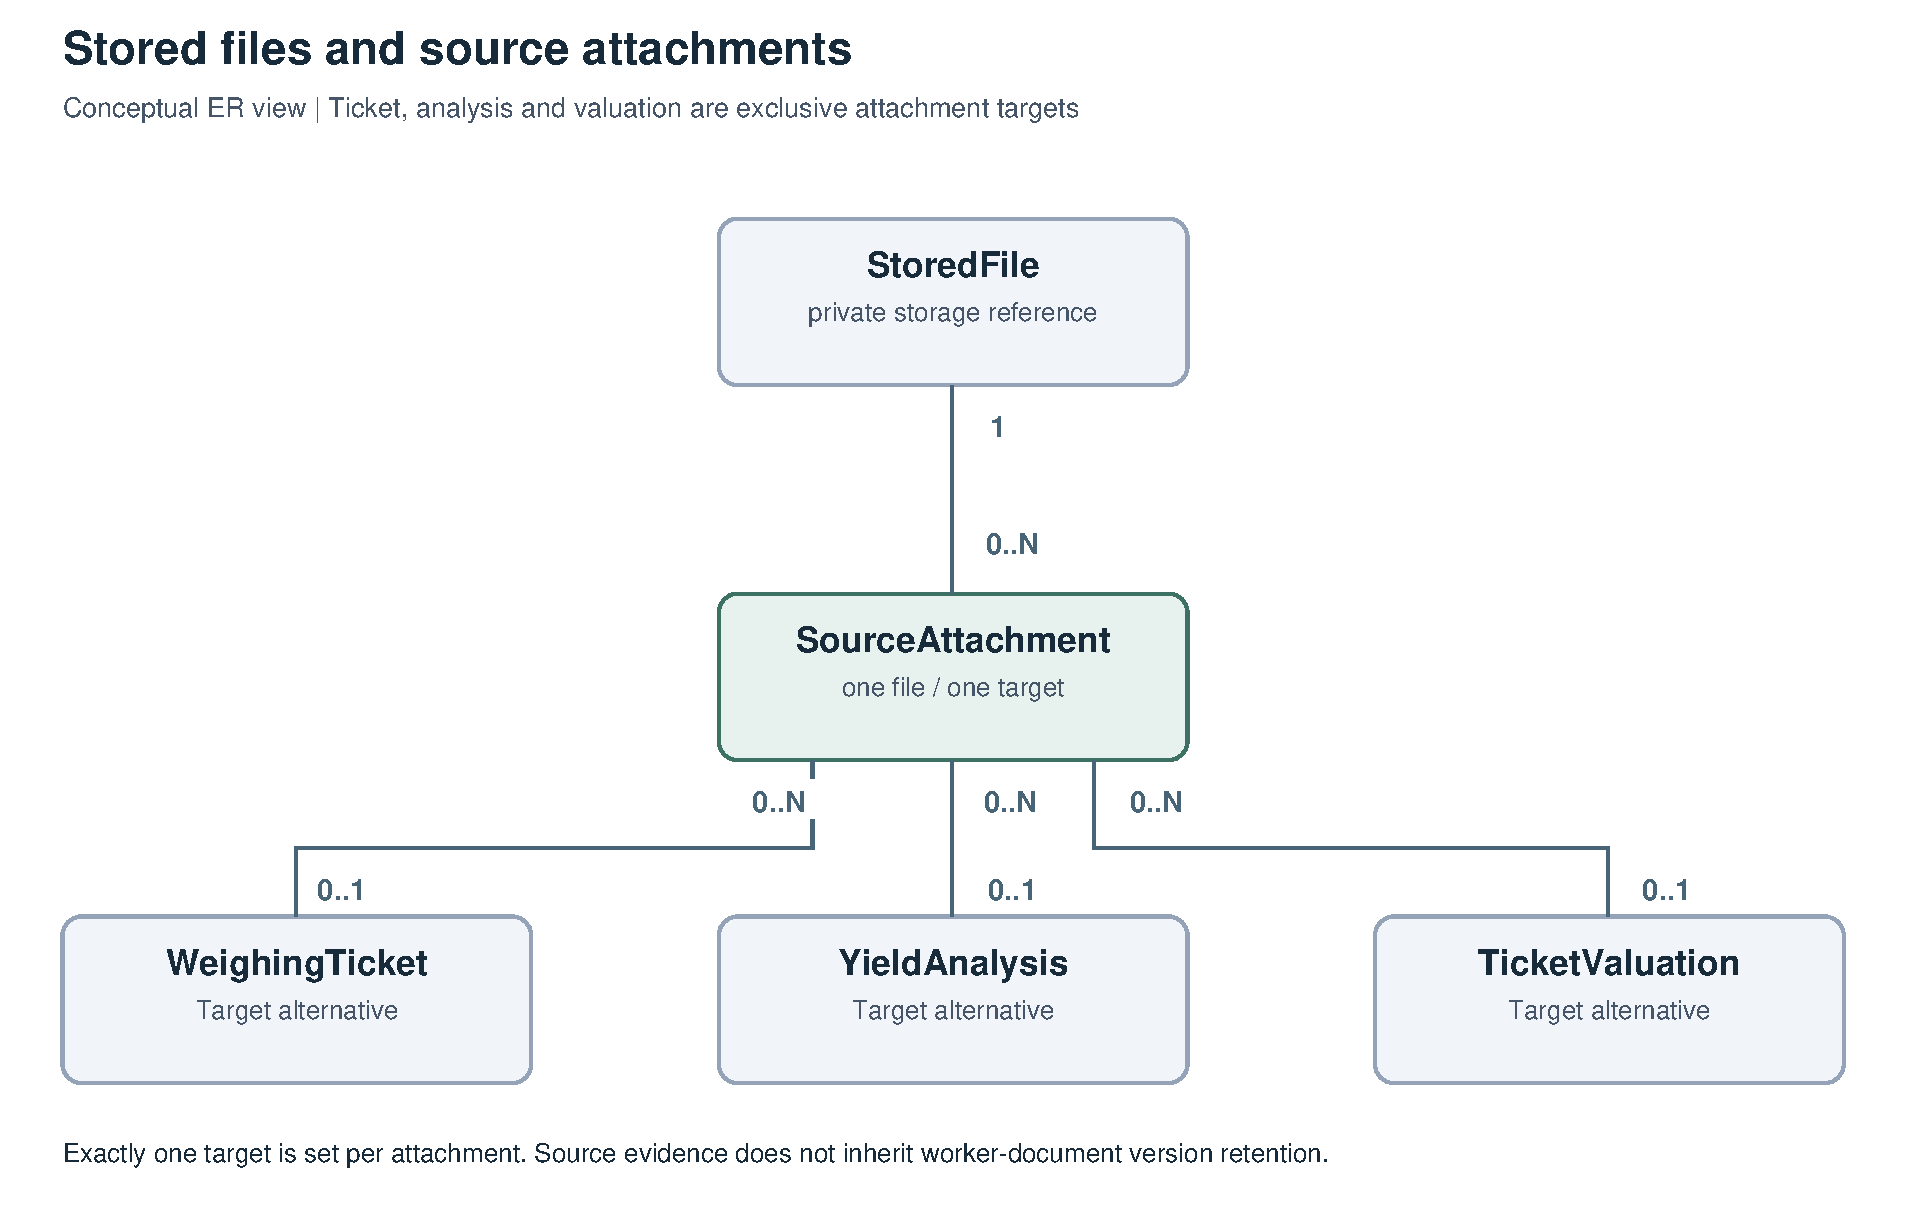
\includegraphics[width=\textwidth]{figures/er-source-files.pdf}
\caption{Source attachments and stored content. Each attachment targets exactly one source record; the three target links are exclusive alternatives.}
\label{fig:er-source-files}
\end{figure}
